\documentclass{article}
% translate with >> pdflatex -shell-escape <file>

\usepackage{pgfplots}
\pgfplotsset{compat=newest}

\pagestyle{empty}

\begin{document}
\begin{tikzpicture}[scale=1.6]%
  \begin{axis}[
      width=.6\textwidth,
      height=0.6\textheight,
      title=Example of Big-$\Omega$,
      ylabel style={overlay},
      yticklabel style={overlay},
      xlabel={$x$},
      ylabel={$y$},
      %legend style={at={(0.5,0.97)},mark=none,
      %   anchor=north,legend columns=-1},
      legend style={ overlay, at={(1.4,.5)}, anchor=center}, every axis plot post/.append style={mark=none},
      domain=-2:6,
      ymax=80
   ]
    \addplot {x^3-4*x^2+x+6};
    \addplot {0.1*x^3};
    \legend{$x^3-4*x^2+x+6$, $0.1*x^3$}
   \end{axis}
\end{tikzpicture}%
\end{document}
